\documentclass[10pt]{article}
\usepackage[margin=1in]{geometry} 
\usepackage{graphicx}
\usepackage{float}
\usepackage{hyperref}
\usepackage{caption}
\usepackage{subcaption}
\usepackage{tcolorbox}
\usepackage{booktabs}
\usepackage{amsmath}
\usepackage{dcolumn}

\title{Final Project: Housing Data Analysis}
\author{Tim Koenders}
\date{\today}
\begin{document}

\maketitle

\tableofcontents 
\listoftables
\listoffigures

\vspace{0.5cm}

\begin{tcolorbox}
\centering \itshape The replication package of this final project is available on GitHub at \href{https://github.com/TimKoenders/Scientific-working-with-R}{https://github.com/TimKoenders/Scientific-working-with-R}.
\end{tcolorbox}

\newpage

\section{Data Description}

\subsection{Variables and Summary Statistics}

The dataset used for this analysis contains information related to housing properties. It includes various attributes that describe different aspects of these properties. The dataset consists of 545 observations and 13 variables. Table~\ref{tab:variables} describes the variable and table~\ref{tab:summary-stats} present the summary statistics for the numeric variables.

\begin{table}[ht]
\centering
\begin{tabular}{@{}ll@{}}
\toprule
\textbf{Variable} & \textbf{Description} \\
\midrule
\textbf{bedrooms} & Number of bedrooms. \\
\textbf{bathrooms} & Number of bathrooms. \\
\textbf{stories} & Number of stories. \\
\textbf{mainroad} & Main road location (yes/no). \\
\textbf{guestroom} & Guestroom presence (yes/no). \\
\textbf{basement} & Basement presence (yes/no). \\
\textbf{hotwaterheating} & Hot water heating (yes/no). \\
\textbf{airconditioning} & Air conditioning (yes/no). \\
\textbf{parking} & Number of parking spaces. \\
\textbf{prefarea} & Preferred area (yes/no). \\
\textbf{furnishingstatus} & Furnishing status. \\
\textbf{area\_m2} & Property area (sq. meters). \\
\textbf{price\_million} & Property price (millions of dollars). \\
\bottomrule
\end{tabular}
\caption{Variable Descriptions}
\label{tab:variables}
\end{table}

\begin{table}[H]
  \centering
  
  \begin{tabular}{lcccccc}
    \toprule
    Variable & Min & 1st Quartile & Median & Mean & 3rd Quartile & Max \\
    \midrule
    bedrooms & 1.000 & 2.000 & 3.000 & 2.965 & 3.000 & 6.000 \\
    bathrooms & 1.000 & 1.000 & 1.000 & 1.286 & 2.000 & 4.000 \\
    stories & 1.000 & 1.000 & 2.000 & 1.806 & 2.000 & 4.000 \\
    parking & 0.0000 & 0.0000 & 0.0000 & 0.6936 & 1.0000 & 3.0000 \\
    area\_m2 & 153.3 & 334.5 & 427.4 & 478.5 & 590.9 & 1505.0 \\
    price\_million & 1.750 & 3.430 & 4.340 & 4.767 & 5.740 & 13.300 \\
    \bottomrule
  \end{tabular}
  \caption{Summary Statistics for Numeric Variables}
  \label{tab:summary-stats}
\end{table}

\subsection{Pairwise Correlations}

I conducted a correlation analysis to understand the relationships between various variables in the data. Table~\ref{tab:3} presents the correlation coefficients. 

\begin{table}[H]
\centering
\begin{tabular}{@{}ccccccc@{}}
\toprule
 & Bedrooms & Bathrooms & Stories & Parking & Area (m$^2$) & Price (Million) \\ \midrule
Bedrooms & 1.0000 & 0.3739 & 0.4086 & 0.1393 & 0.1519 & 0.3665 \\
Bathrooms & 0.3739 & 1.0000 & 0.3262 & 0.1775 & 0.1938 & 0.5175 \\
Stories & 0.4086 & 0.3262 & 1.0000 & 0.0455 & 0.0840 & 0.4207 \\
Parking & 0.1393 & 0.1775 & 0.0455 & 1.0000 & 0.3530 & 0.3844 \\
Area (m$^2$) & 0.1519 & 0.1938 & 0.0840 & 0.3530 & 1.0000 & 0.5360 \\
Price (Million) & 0.3665 & 0.5175 & 0.4207 & 0.3844 & 0.5360 & 1.0000 \\ \bottomrule
\end{tabular}
\caption{Correlation Matrix}
\label{tab:3}
\end{table}

The correlation analysis reveals several interesting insights. The number of bedrooms and bathrooms exhibits a positive correlation of approximately 0.374. This suggests that properties with more bedrooms are likely to have more bathrooms, which is a common expectation in residential real estate. In contrast, the correlation between parking spaces and other variables is relatively weak. Notably, the strongest correlation in the data is observed between the price in a million dollars and the area in square meters, with a coefficient of 0.5360. This indicates that the price of residential properties tends to increase notably with the area in squared meters, as intuition would suggest. Overall, the correlation analysis provides valuable insights into the linear relationships between variables in the data.

\subsection{Visualizations}

Figure~\ref{fig:1}  provides valuable insights into the relationship between property area and price and the impact of furnishing status on property values. The scatter plot in Figure~\ref{fig:1a} clearly illustrates a positive correlation between the area in squared meters and property price. As the area increases, so does the property's market value, which aligns with our expectations. In Figure~\ref{fig:1b}, the box plots of transformed prices categorised by furnishing status reveal interesting trends. Furnished or semi-furnished properties tend to command higher prices on average compared to their unfurnished counterparts. This suggests that the level of furnishing is an essential factor influencing property prices in our data. In Figure~\ref{fig:2}, we focus on property attributes such as the number of bedrooms and their relationship with the property's location. In Figure~\ref{fig:2a}, the histogram of bedrooms provides a distribution of the number of bedrooms in our data. This can help us identify the most common bedroom counts in the properties. Figure~\ref{fig:2b} compares properties located on the main road and those not on the main road concerning air conditioning. The bar chart shows that properties situated on the main road are more likely to have air conditioning compared to those located off the main road. This insight could be valuable for potential buyers or investors looking for specific amenities in their desired property location.

\begin{figure}[H]
  \centering
  \begin{subfigure}{0.3\textwidth}
    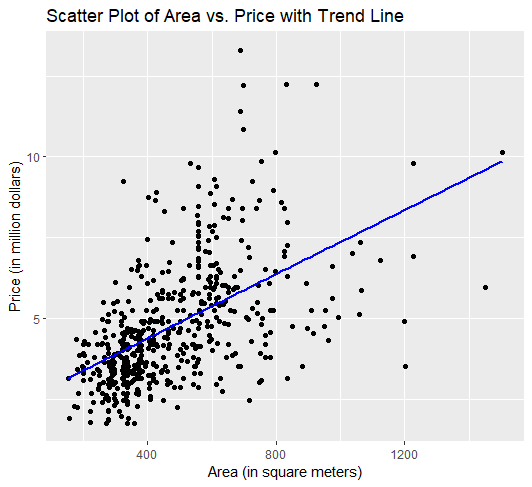
\includegraphics[width=\linewidth]{Final project/Visualizations/Scatterplot.png}
    \caption{Scatter Plot of Area vs. Transformed Price}
    \label{fig:1a}
  \end{subfigure}
  \begin{subfigure}{0.3\textwidth}
    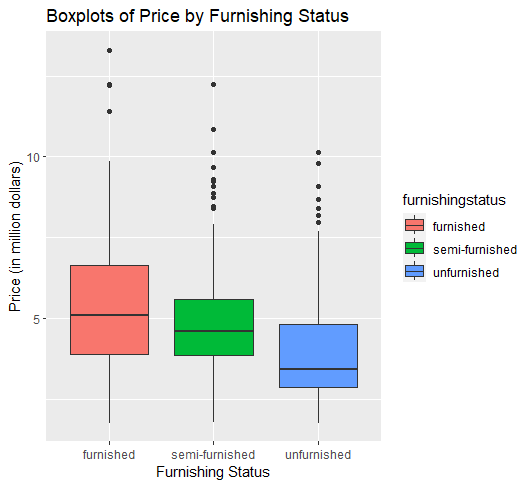
\includegraphics[width=\linewidth]{Final project/Visualizations/Boxplot.png}
    \caption{Box plots of Price by Furnishing Status}
    \label{fig:1b}
  \end{subfigure}
  \caption{Scatter plot and box plot}
  \label{fig:1}
\end{figure}

\begin{figure}[H]
  \centering
  \begin{subfigure}{0.25\textwidth}
    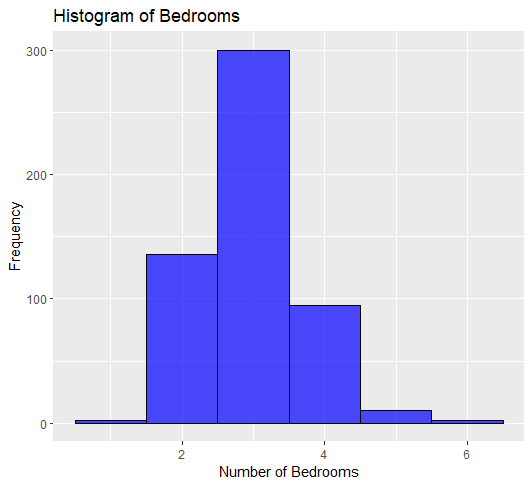
\includegraphics[width=\linewidth]{Final project/Visualizations/Histogram.png}
    \caption{Histogram of bedrooms}
    \label{fig:2a}
  \end{subfigure}
  \begin{subfigure}{0.25\textwidth}
    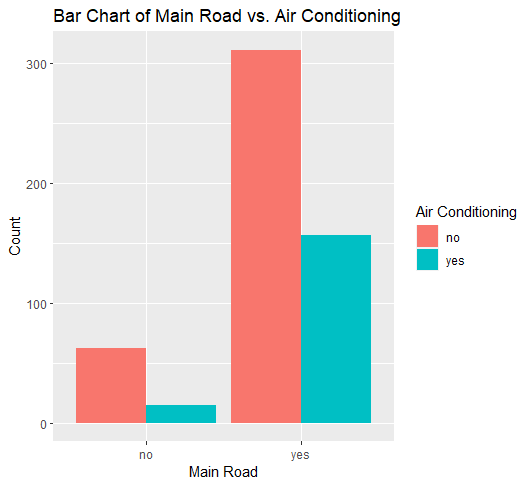
\includegraphics[width=\linewidth]{Final project/Visualizations/Bar chart.png}
    \caption{Bar chart of main road vs. air conditioning}
    \label{fig:2b}
  \end{subfigure}
  \caption{Additional visualizations}
  \label{fig:2}
\end{figure}

\section{Linear Regression}

In the context of OLS regression, we express the relationship between housing prices and multiple explanatory variables as follows:

\begin{equation}
y_i = X_{i}'\beta + \epsilon_i
\end{equation}

where $y_i$ represents the housing prices in millions, $X_{i}$ is a vector of explanatory variables and $\epsilon_i$ denotes a nonsystematic error term. In Figure~\ref{fig:3}, we present a scatter plot visually illustrating the relationship between actual housing prices and their corresponding predicted values. The scatter plot reveals a pronounced positive correlation, indicating that our regression model effectively captures and replicates the real-world dynamics of housing prices. This alignment between actual and predicted values underscores the model's robustness in explaining variations in housing prices and signifies its utility as a predictive tool for real estate valuation. Table~\ref{tab:4} shows the results of the OLS estimation. The number of bathrooms and stories impact housing prices significantly. Moreover, primary road access, the presence of a guestroom, a basement, hot water heating, air conditioning, and parking spots also significantly positively impact housing prices. There is no significant difference in housing prices between semi-furnished and furnished houses. Still, housing prices are, on average, lower for unfurnished houses compared to furnished houses. Contrary to my expectations, the number of bedrooms is not an important predictor of housing prices, likely due to the severe multicollinearity in the data. This motivates the use of lasso regression in the next section. Finally, the area of the property is also a significant predictor of housing prices. An additional square meter is expected to increase housing prices by 3,000 dollars. 

\begin{figure}[H]
  \centering
  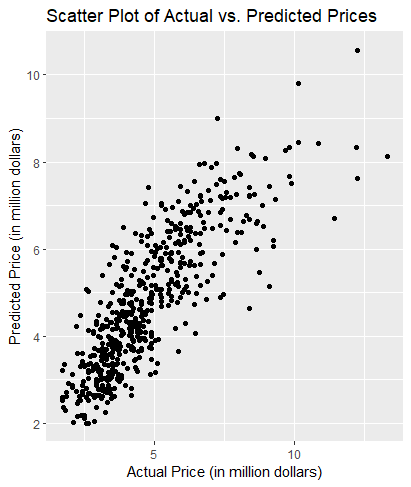
\includegraphics[width=0.6\linewidth]{Final project/Visualizations/Scatterplot_2.png}
  \caption{Scatter Plot of Actual vs. Predicted Transformed Prices}
   \label{fig:3}
\end{figure}

\begin{table}[H] \centering 
\renewcommand{\arraystretch}{0.8} % Reduce line spacing for better fit
 \caption{Linear Regression Results} 
  \label{tab:4}
\begin{tabular}{@{\extracolsep{5pt}}lD{.}{.}{-3} } 
\\[-1.8ex]\hline 
\hline \\[-1.8ex] 
 & \multicolumn{1}{c}{\textit{Dependent variable:}} \\ 
\cline{2-2} 
\\[-1.8ex] & \multicolumn{1}{c}{price\_million} \\ 
\hline \\[-1.8ex] 
 bedrooms & 0.115 \\ 
  & (0.073) \\ 
  & \\ 
 bathrooms & 0.988^{***} \\ 
  & (0.103) \\ 
  & \\ 
 stories & 0.451^{***} \\ 
  & (0.064) \\ 
  & \\ 
 mainroadyes & 0.421^{***} \\ 
  & (0.142) \\ 
  & \\ 
 guestroomyes & 0.301^{**} \\ 
  & (0.132) \\ 
  & \\ 
 basementyes & 0.350^{***} \\ 
  & (0.110) \\ 
  & \\ 
 hotwaterheatingyes & 0.855^{***} \\ 
  & (0.223) \\ 
  & \\ 
 airconditioningyes & 0.865^{***} \\ 
  & (0.108) \\ 
  & \\ 
 parking & 0.277^{***} \\ 
  & (0.059) \\ 
  & \\ 
 prefareayes & 0.652^{***} \\ 
  & (0.116) \\ 
  & \\ 
 furnishingstatussemi-furnished & -0.046 \\ 
  & (0.117) \\ 
  & \\ 
 furnishingstatusunfurnished & -0.411^{***} \\ 
  & (0.126) \\ 
  & \\ 
 area\_m2 & 0.003^{***} \\ 
  & (0.0003) \\ 
  & \\ 
 Constant & 0.043 \\ 
  & (0.264) \\ 
  & \\ 
\hline \\[-1.8ex] 
Observations & \multicolumn{1}{c}{545} \\ 
R$^{2}$ & \multicolumn{1}{c}{0.682} \\ 
Adjusted R$^{2}$ & \multicolumn{1}{c}{0.674} \\ 
Residual Std. Error & \multicolumn{1}{c}{1.068 (df = 531)} \\ 
F Statistic & \multicolumn{1}{c}{87.521$^{***}$ (df = 13; 531)} \\ 
\hline 
\hline \\[-1.8ex] 
\textit{Note:}  & \multicolumn{1}{r}{$^{*}$p$<$0.1; $^{**}$p$<$0.05; $^{***}$p$<$0.01} \\ 
\end{tabular} 
\end{table} 

\section{LASSO Regression}

Table~\ref{tab:lasso-results} displays the estimation results of the LASSO estimation. Several predictors are set to zero. These excluded predictors are considered non-informative or unimportant for predicting the target variable, and Lasso helps with feature selection. The LASSO results indicate that the number of bathrooms, stories, air conditioning and area positively affect housing prices. 

\begin{table}[H]
\centering
\begin{tabular}{lcc}
\hline
\textbf{Variable} & \textbf{Coefficient} \\
\hline
Intercept & 2.314 \\
bedrooms & - \\
bathrooms & 0.653 \\
stories & 0.111 \\
mainroad & - \\
guestroom & - \\
basement & - \\
hotwaterheating & - \\
airconditioning & 0.365 \\
parking & - \\
prefarea & - \\
furnishingstatus & - \\
area\_m2 & 0.002 \\
\hline
\end{tabular}
\caption{Lasso Regression Results}
\label{tab:lasso-results}
\end{table}


\begin{figure}[H]
\renewcommand{\arraystretch}{0.6} % Reduce line spacing for better fit
  \centering
  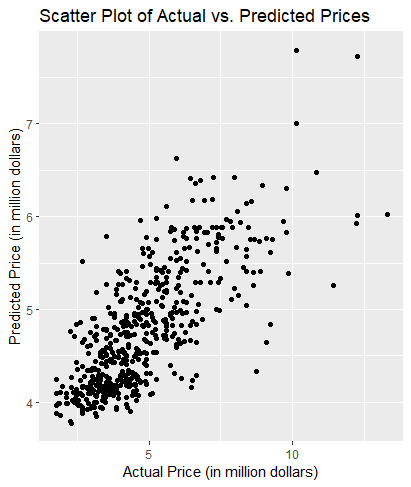
\includegraphics[width=0.6\linewidth, height=0.5\linewidth]{Final project/Visualizations/Scatterplot3.png}
  \caption{Scatter Plot of Actual vs. Predicted Transformed Prices (LASSO Model)}
  \label{fig:4}
\end{figure}



\section{Conclusion}

Our analysis unveiled valuable insights into the interrelationships among housing property attributes. Notably, we found strong positive correlations between property area and price and between the number of bathrooms and price. Visualisations provided additional clarity, including scatter plots, box plots, histograms, and bar charts. These visuals illustrated correlations, the impact of furnishing status on property values, and distributions of key attributes. For predicting housing prices, linear regression proved informative, highlighting significant predictors like the number of bathrooms, stories, and air conditioning. Property area also played a substantial role in price determination. Incorporating LASSO regression facilitated feature selection, refining the model by retaining essential predictors. In summary, our project offered a brief analysis of housing data, shedding light on factors influencing property prices. Our regression models explained price variations and underscored the significance of specific variables.  Future research and model refinement could enhance predictive accuracy for housing prices.


\end{document}
